\documentclass[12pt,oneside]{article}
\usepackage{graphicx} % Allows including images
\usepackage{hanging}
%\usepackage{hyperref}
\addtolength{\textwidth}{3cm}
\addtolength{\oddsidemargin}{-1.5cm}
\addtolength{\textheight}{4cm}
\addtolength{\topmargin}{-2cm}
%\setlength{\parskip}{-1em}
%\setlength\parskip{0em plus 0.1em minus 0.2em}
\newcommand{\pdv}[2]{\frac{\partial \, #1}{\partial #2}}
\newcommand{\ol}{\overline}
\newcommand{\p}{\partial}
\newcommand{\etal}{ {\it et al.} }
\pagestyle{empty}
\begin{document}


A simple planar profile is utilized, as shown in Fig \ref{fig1}.
\begin{figure}
  \begin{center}
    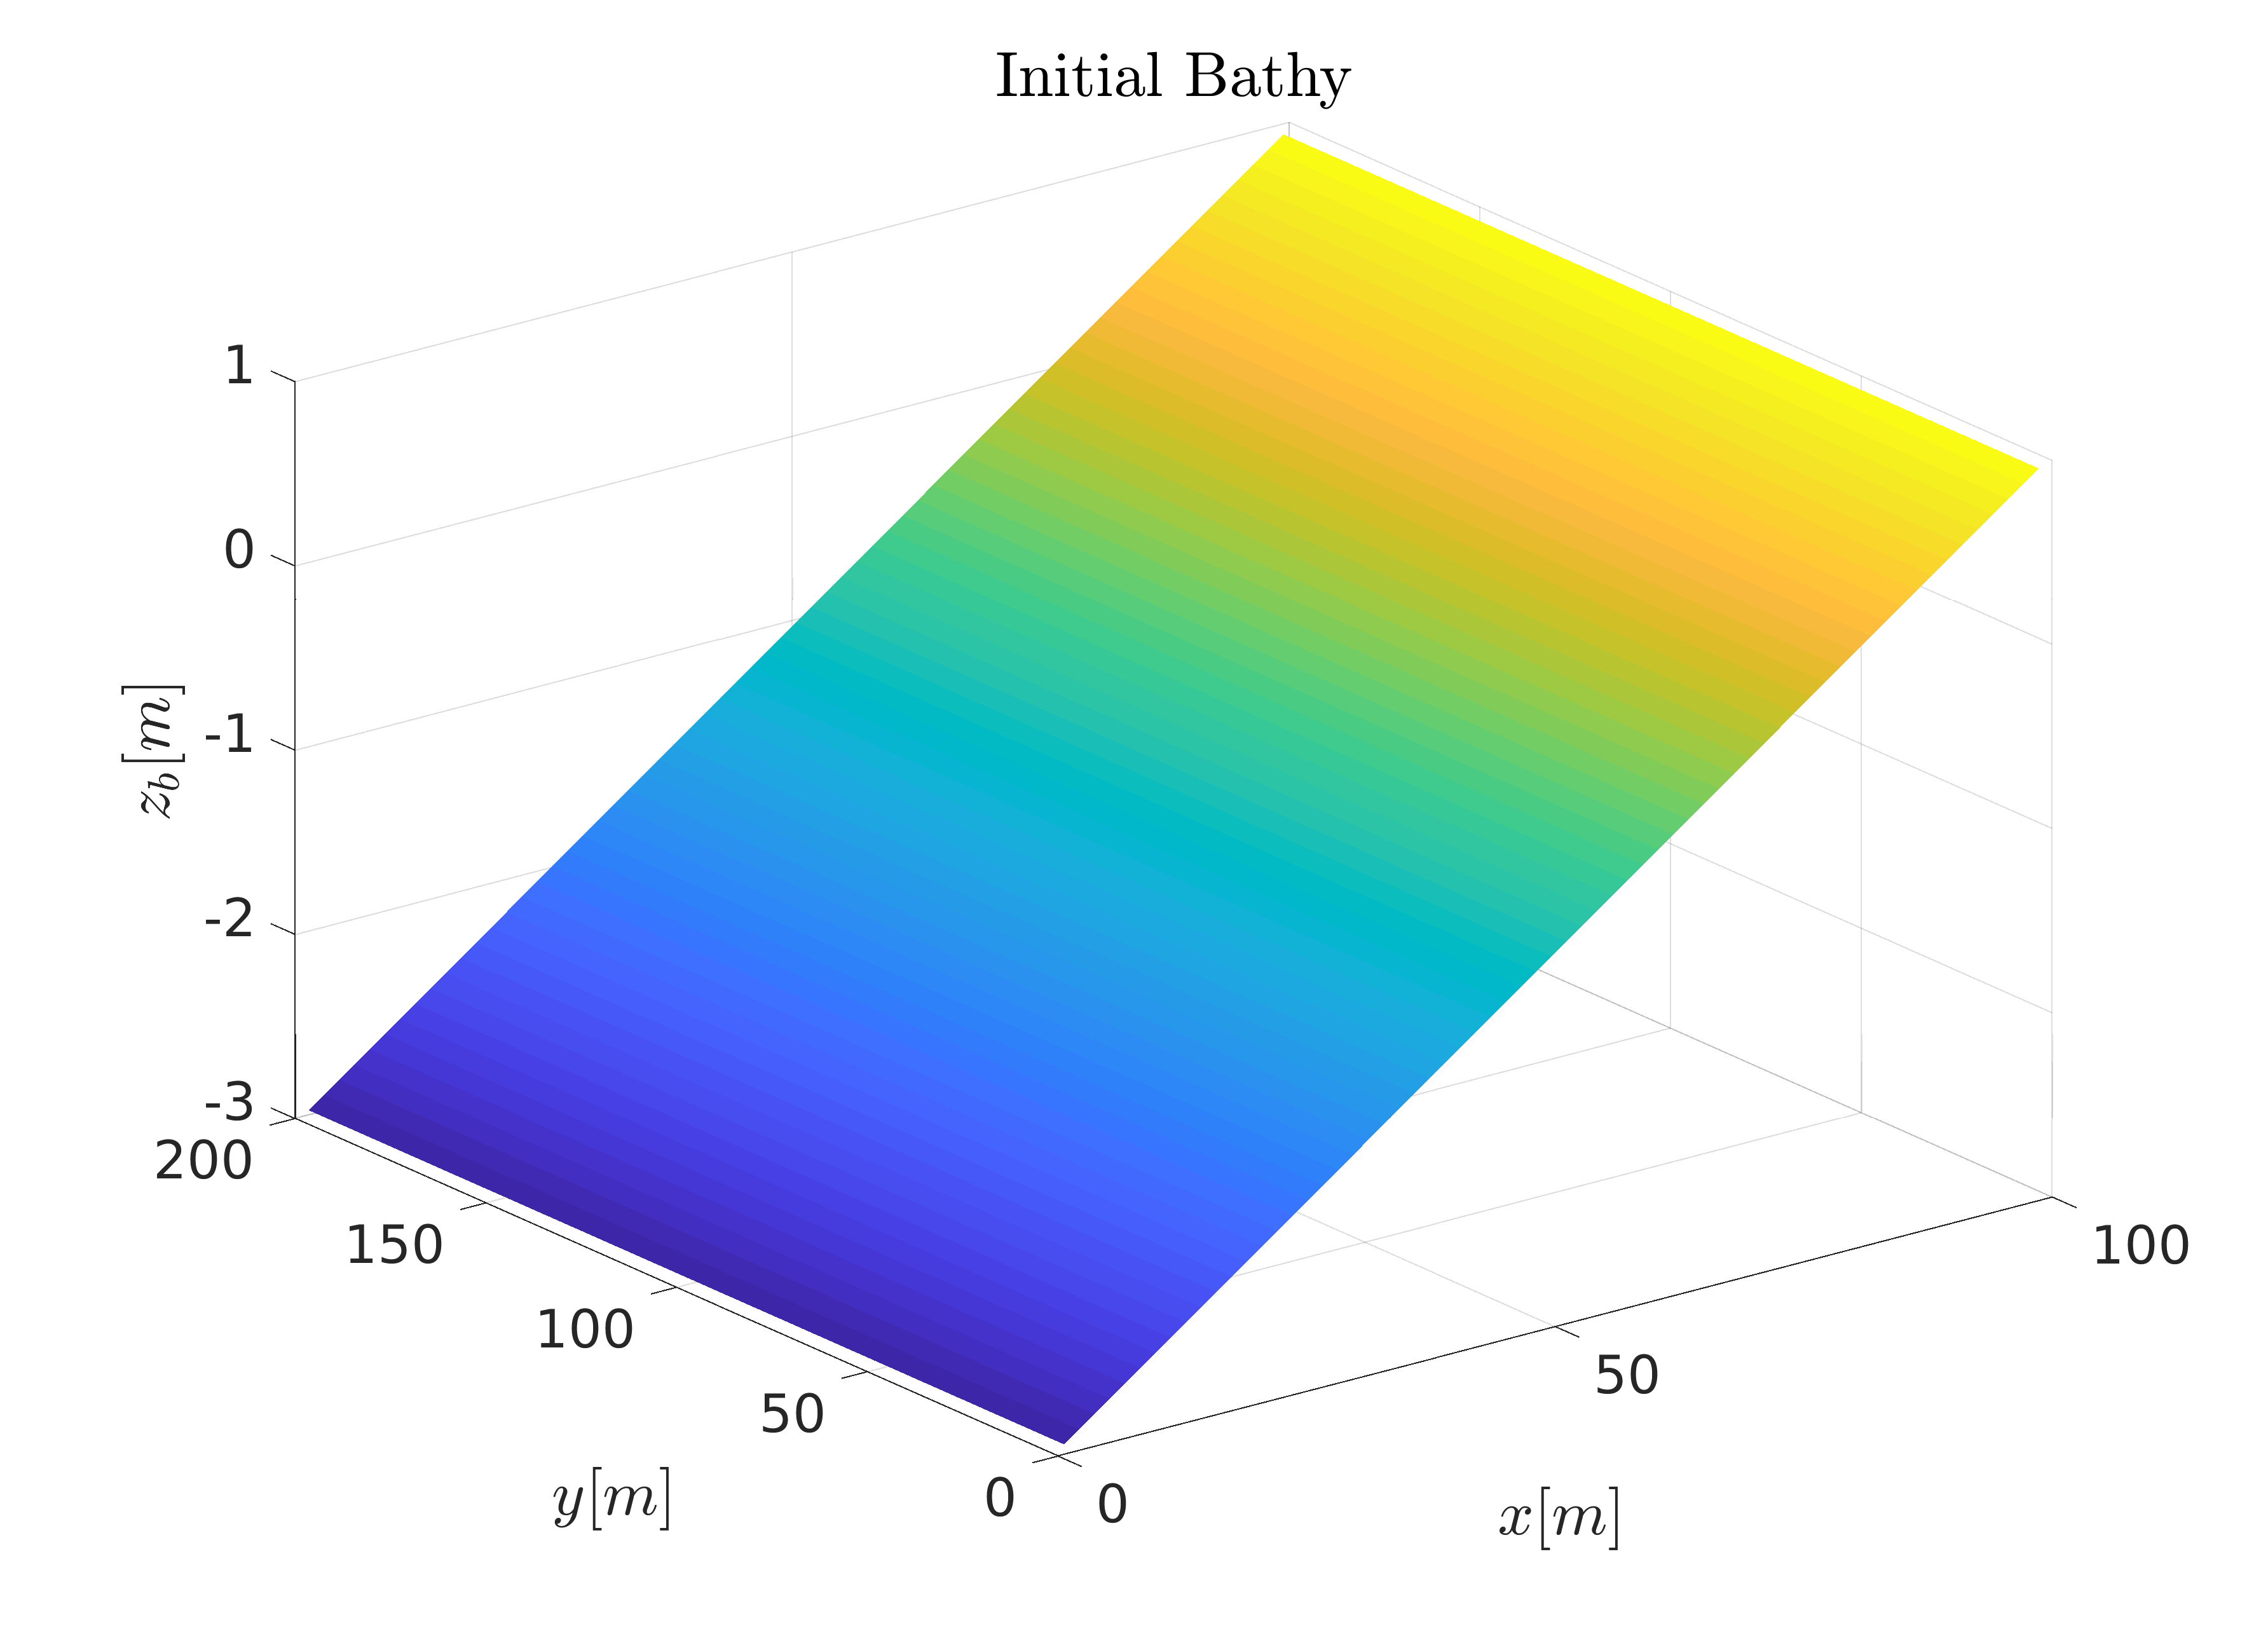
\includegraphics[width=.8\linewidth]{./zb_init.png}
  \end{center}
  \caption{Planar profile}
  \label{fig1}
\end{figure}
Normally incident waves of $H_{rms} = 1m$ and $T= 8s$ are run for 3 hours.  With
\begin{verbatim}
 WAVE_INDUCED_SED_TRANS              OFF
\end{verbatim}
and using the Lund-CIRP formulation, the transport field is shown in
Fig \ref{fig2}.  In this simulation without wave-driven impacts, transport
is in accordance with simple current advection.
\begin{figure}
  \begin{center}
    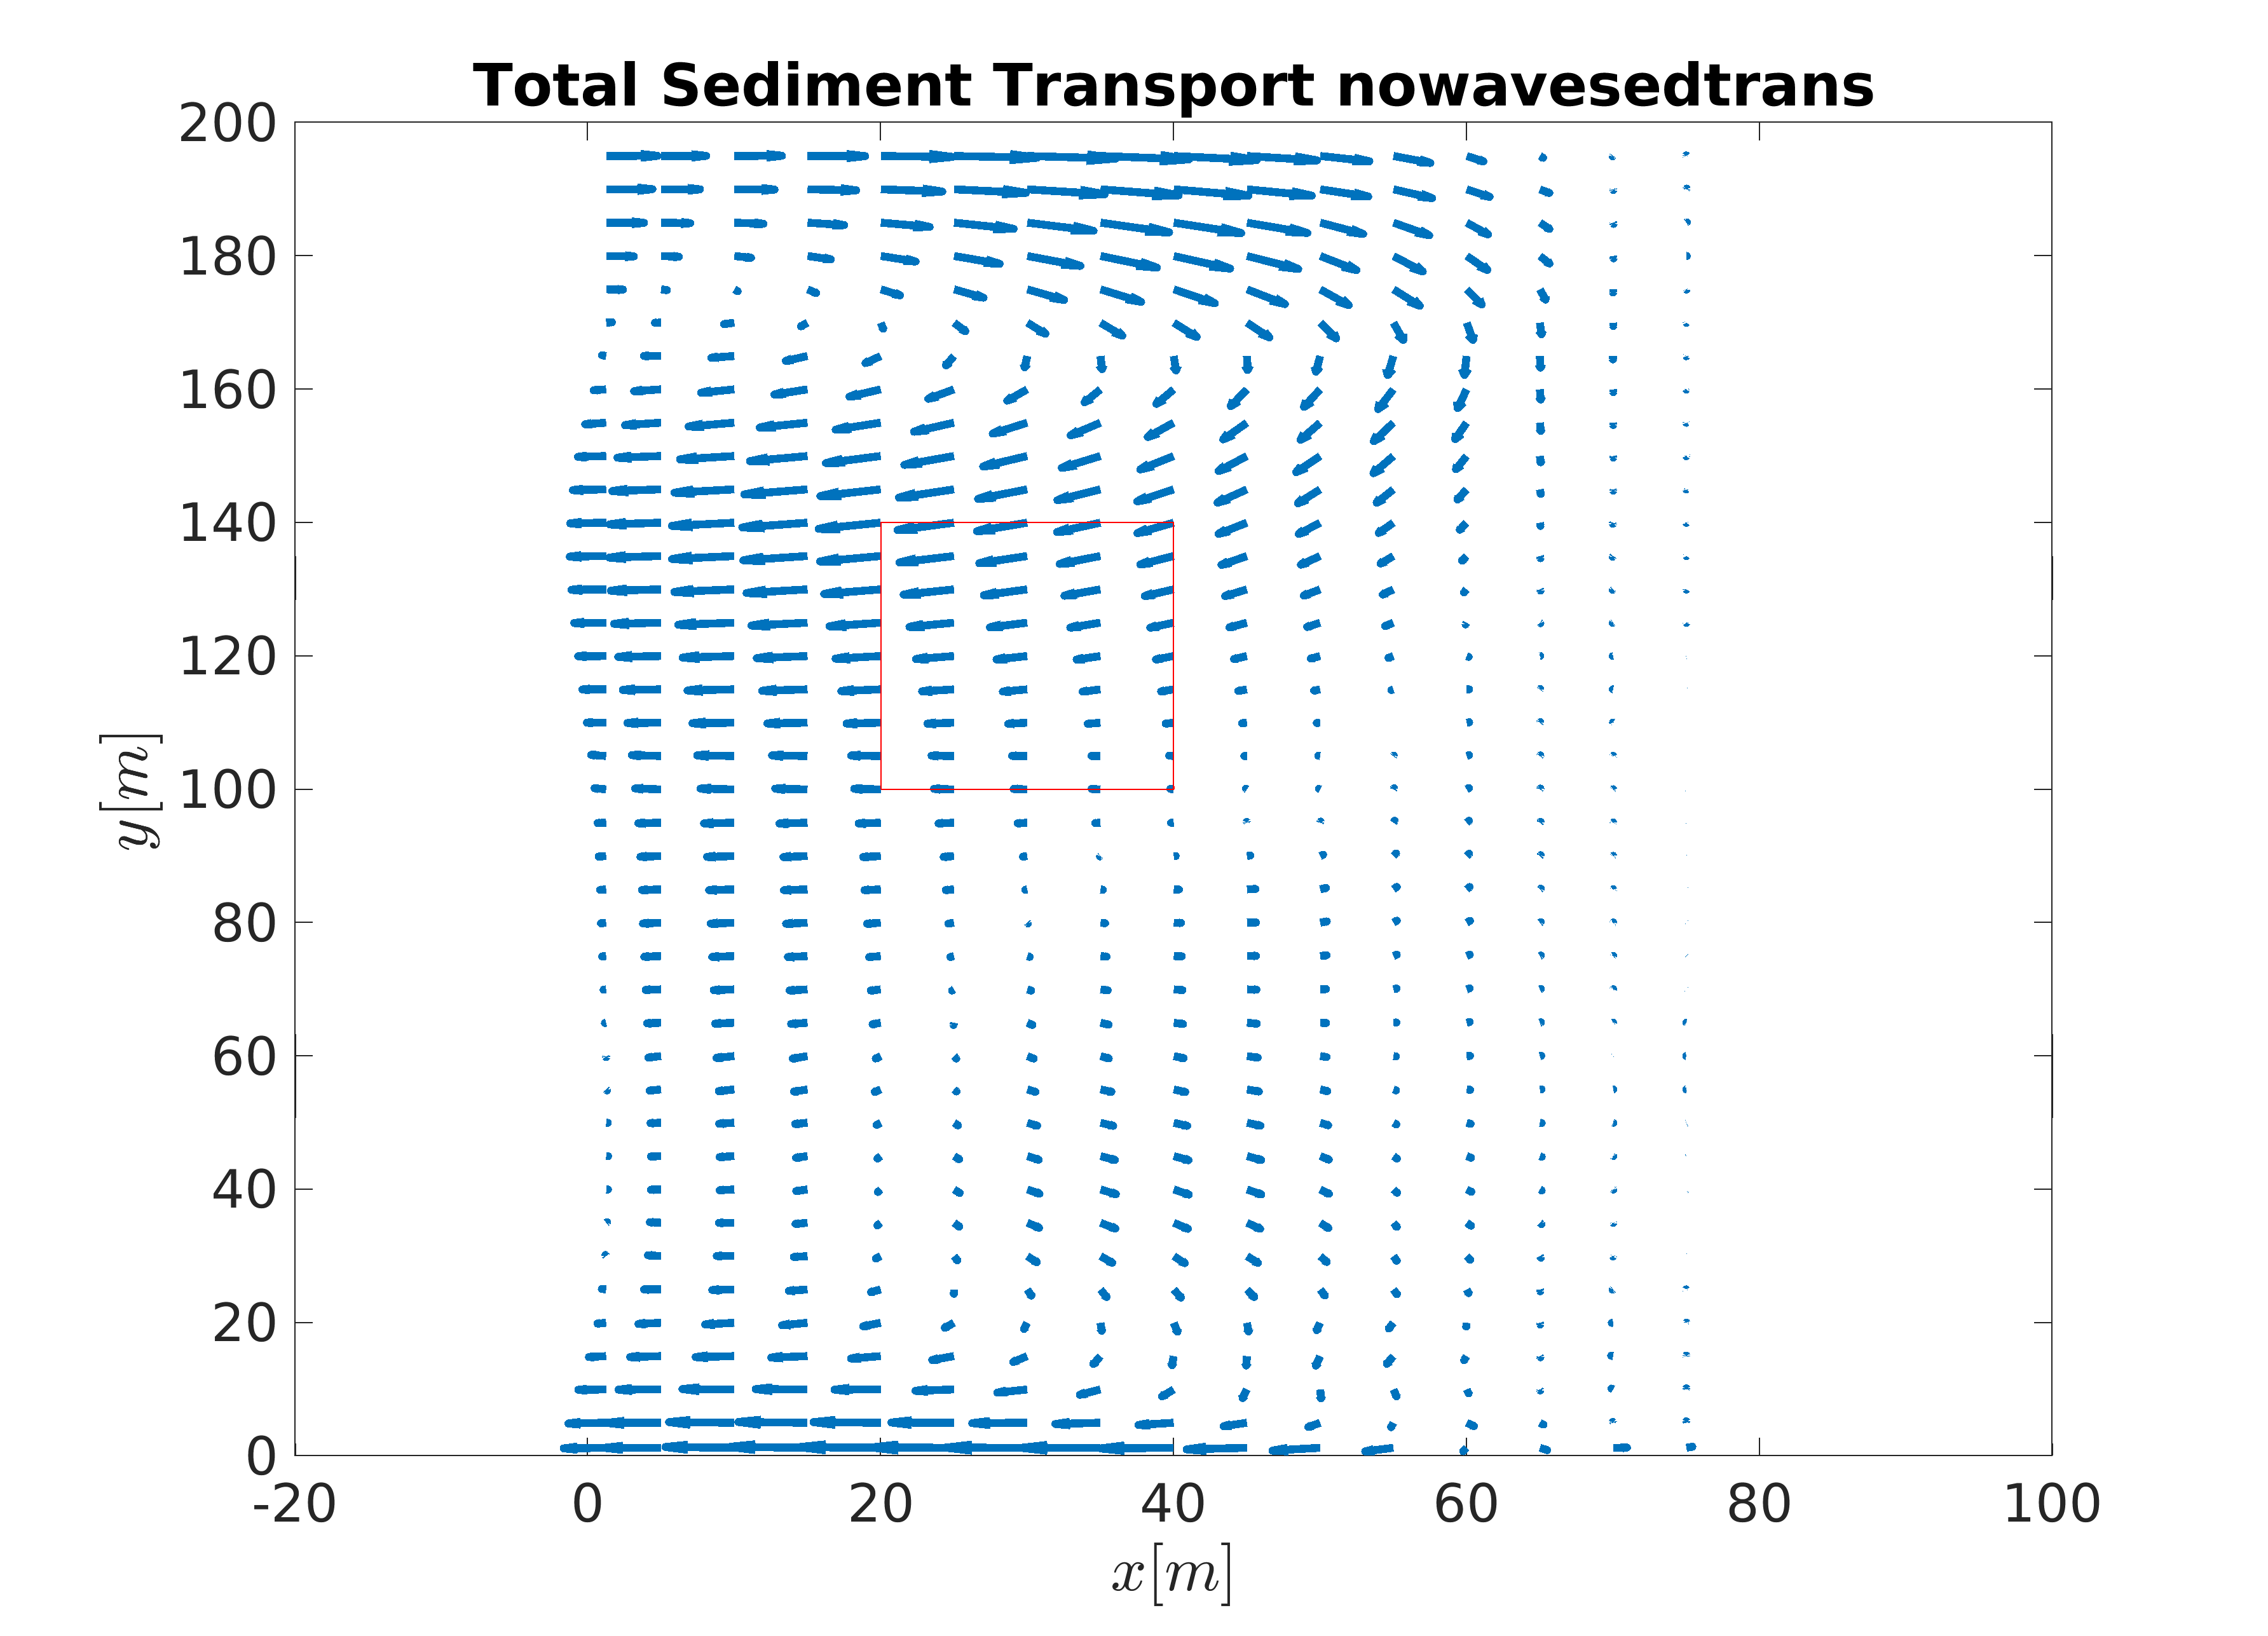
\includegraphics[width=.8\linewidth]{./transport_vec_nowavesedtrans.png}
  \end{center}
  \caption{Transport field}
  \label{fig2}
\end{figure}
The red box depicted in the field will act as a control volume for a
rough check.  Twice integrating the sand conservation statement in
$x,y$ and again in time results in a time series for volume in the box
where changes in volume are balanced by the cumulative sum total of transport
across the boundary.
\begin{figure}
  \begin{center}
    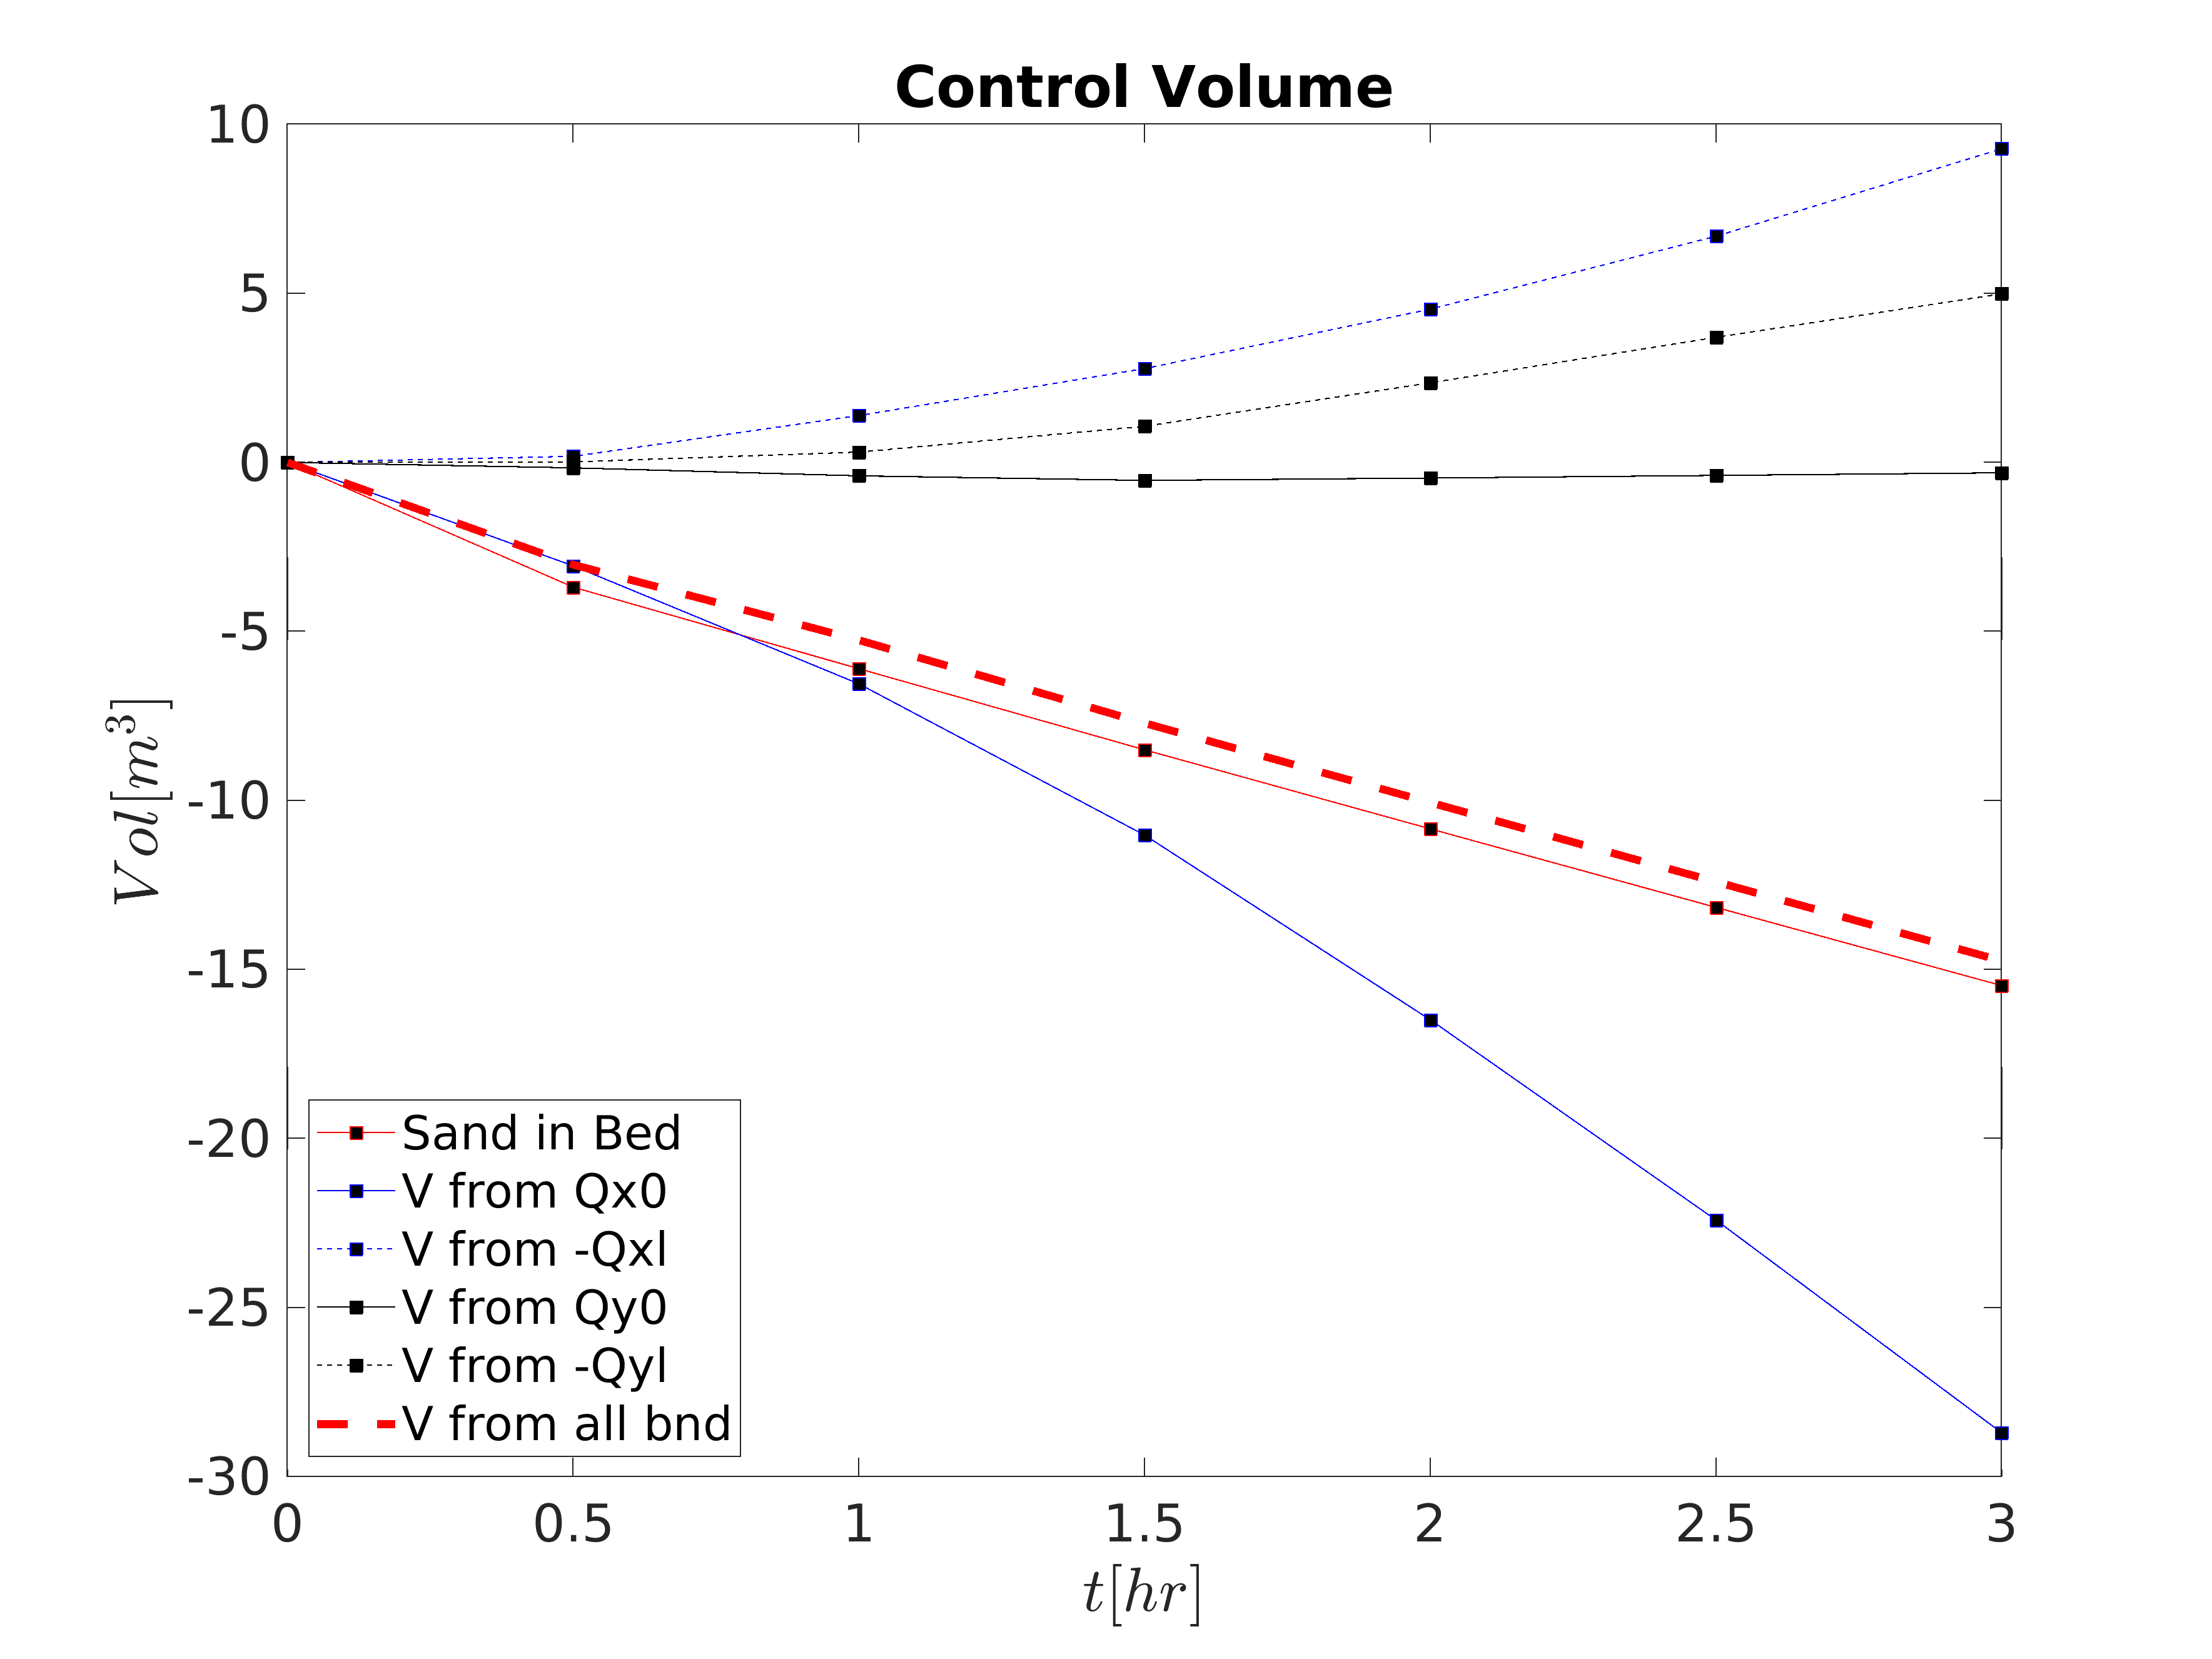
\includegraphics[width=.8\linewidth]{./control_volnowavesedtrans.png}
  \end{center}
  \caption{Control Volume}
  \label{fig3}
\end{figure}
Figure \ref{fig3} shows the time-series of box volume as a solid red
line and the total cumulative transport across boundaries as a dashed
red line.  The analysis is somewhat simplified, herein, using low-order
numerical integration in time and space, and so the expectation is
that the red lines are approximately coincident, as shown.  
\clearpage

Alternatively, with 
\begin{verbatim}
 WAVE_INDUCED_SED_TRANS              ON
\end{verbatim}
the transport field is shown in
Fig \ref{fig2} where wave-driven transport is exaggerated and onshore.
\begin{figure}
  \begin{center}
    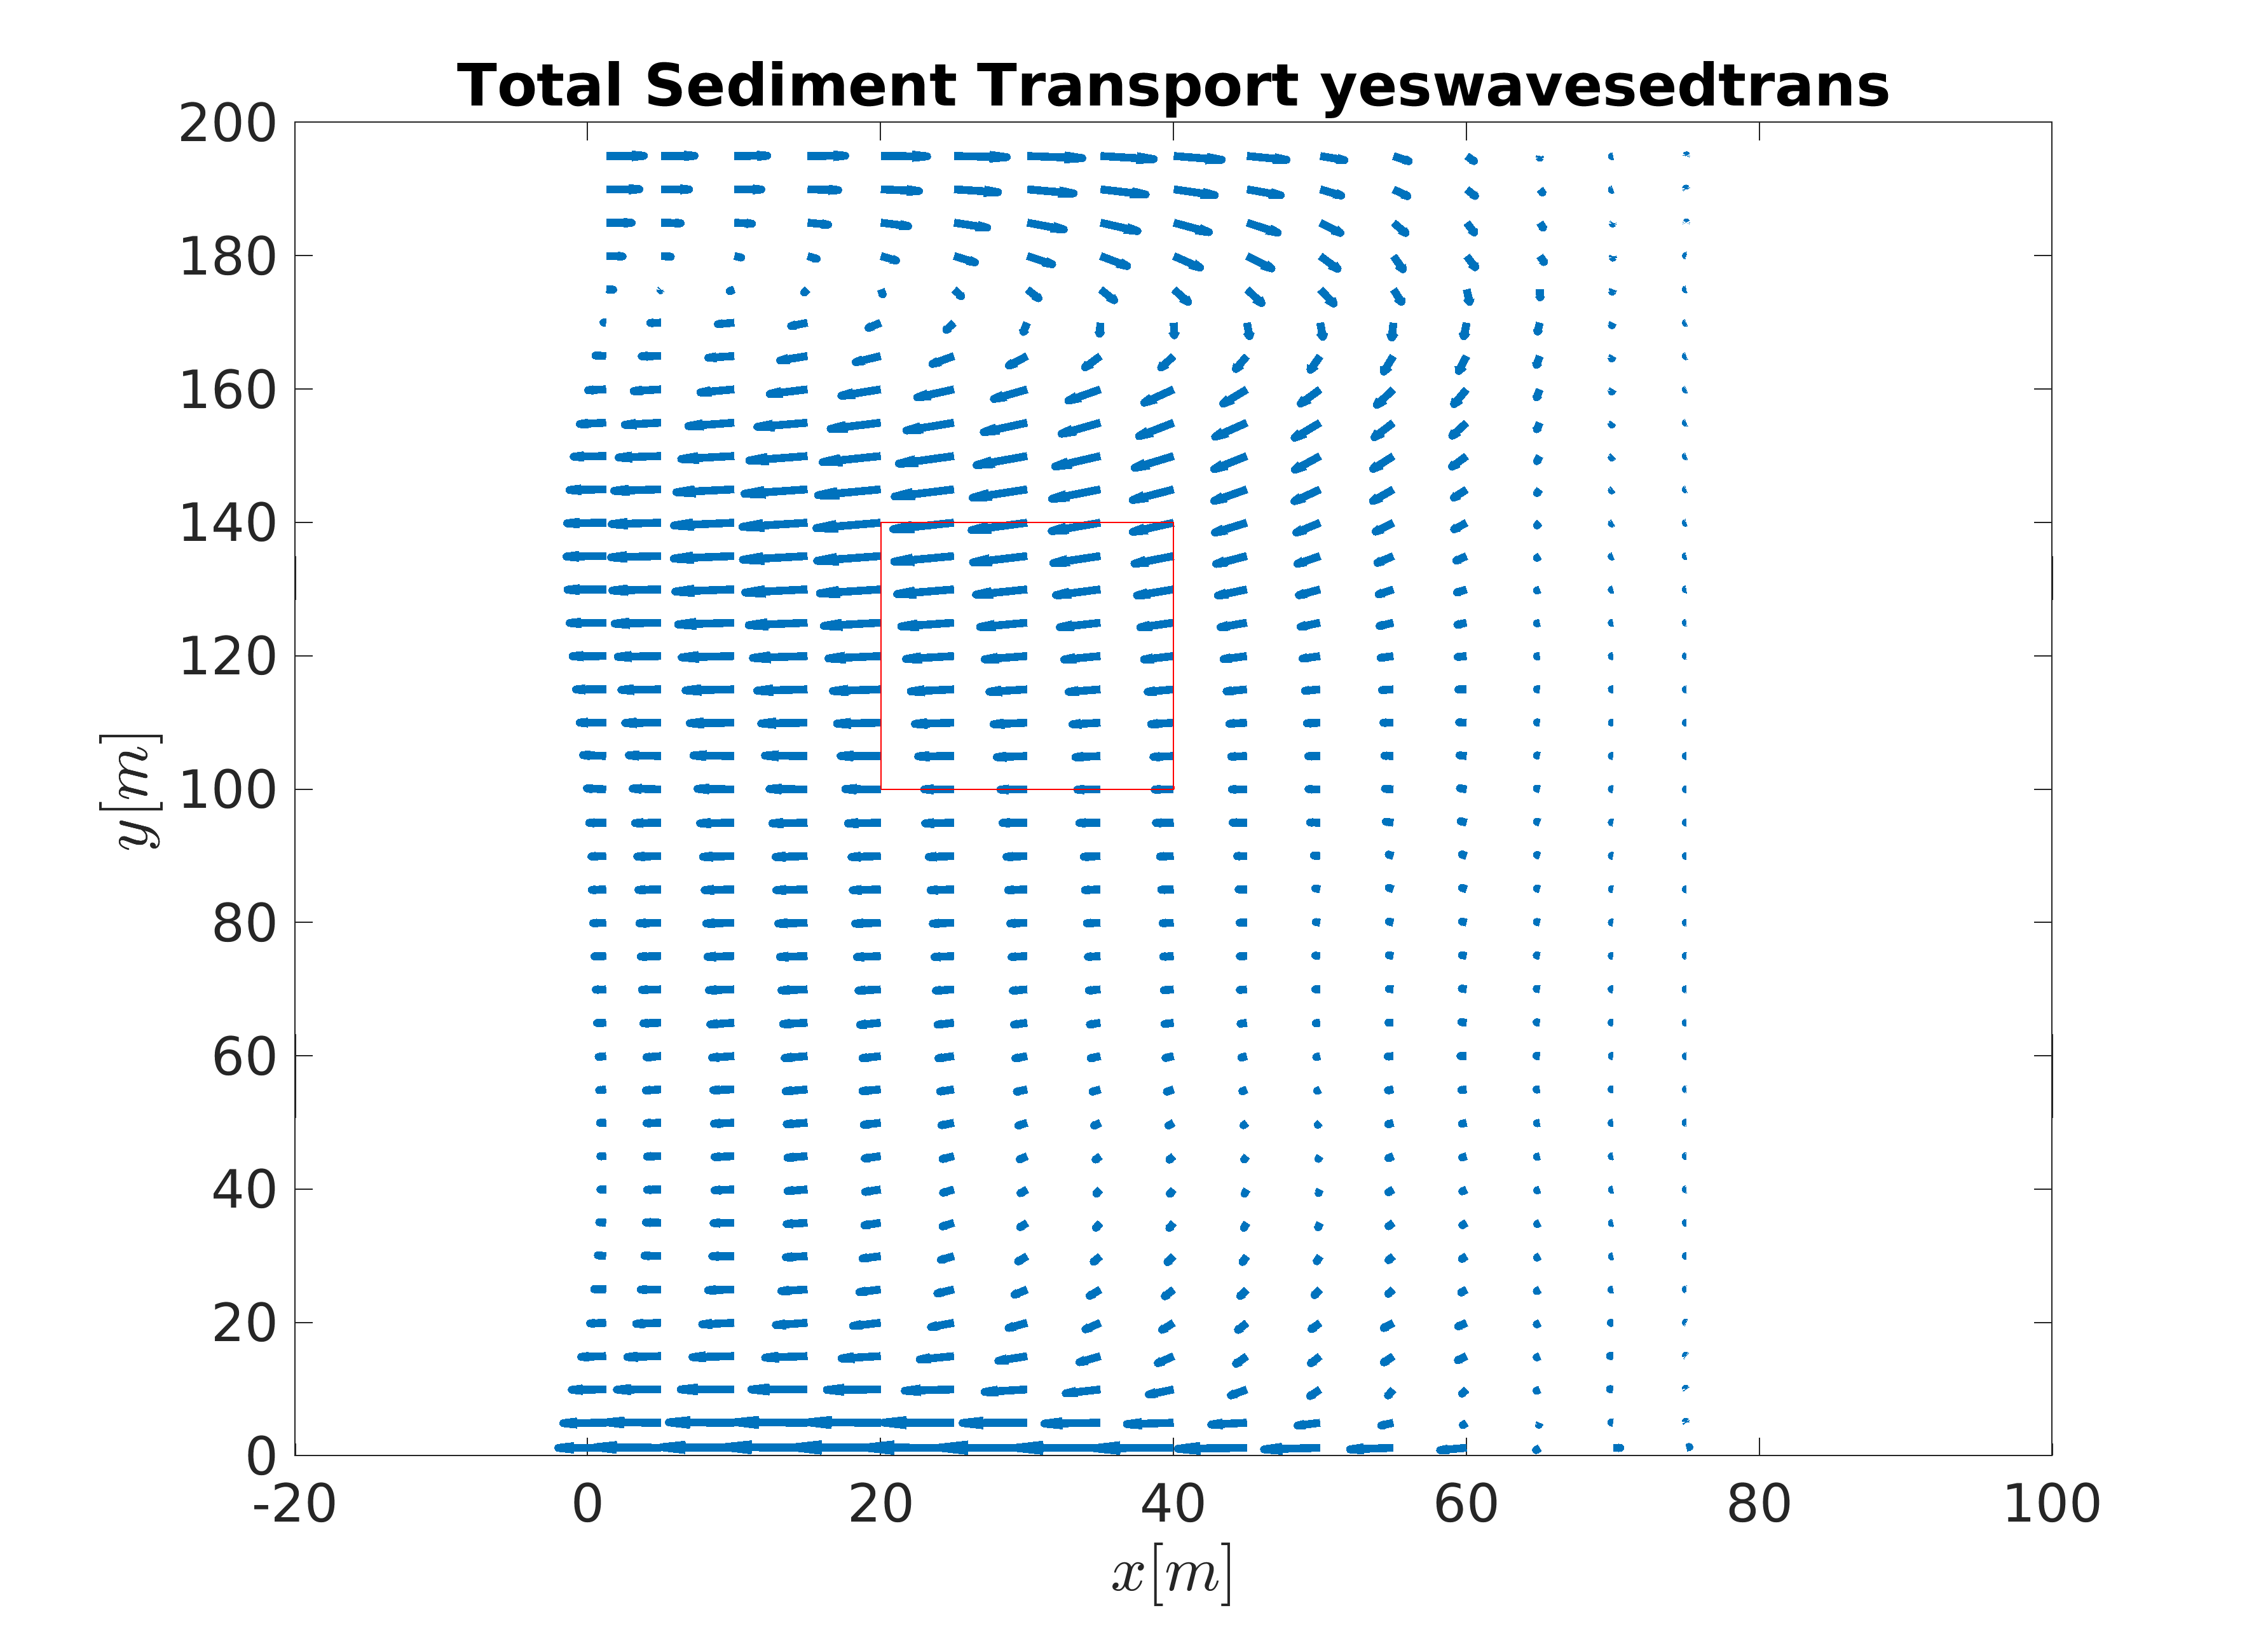
\includegraphics[width=.8\linewidth]{./transport_vec_yeswavesedtrans.png}
  \end{center}
  \caption{Transport field}
  \label{fig4}
\end{figure}
The analogous control volume analysis is provided in Fig \ref{fig5}, where the difference in volume and boundary flux are obvious.
\begin{figure}
  \begin{center}
    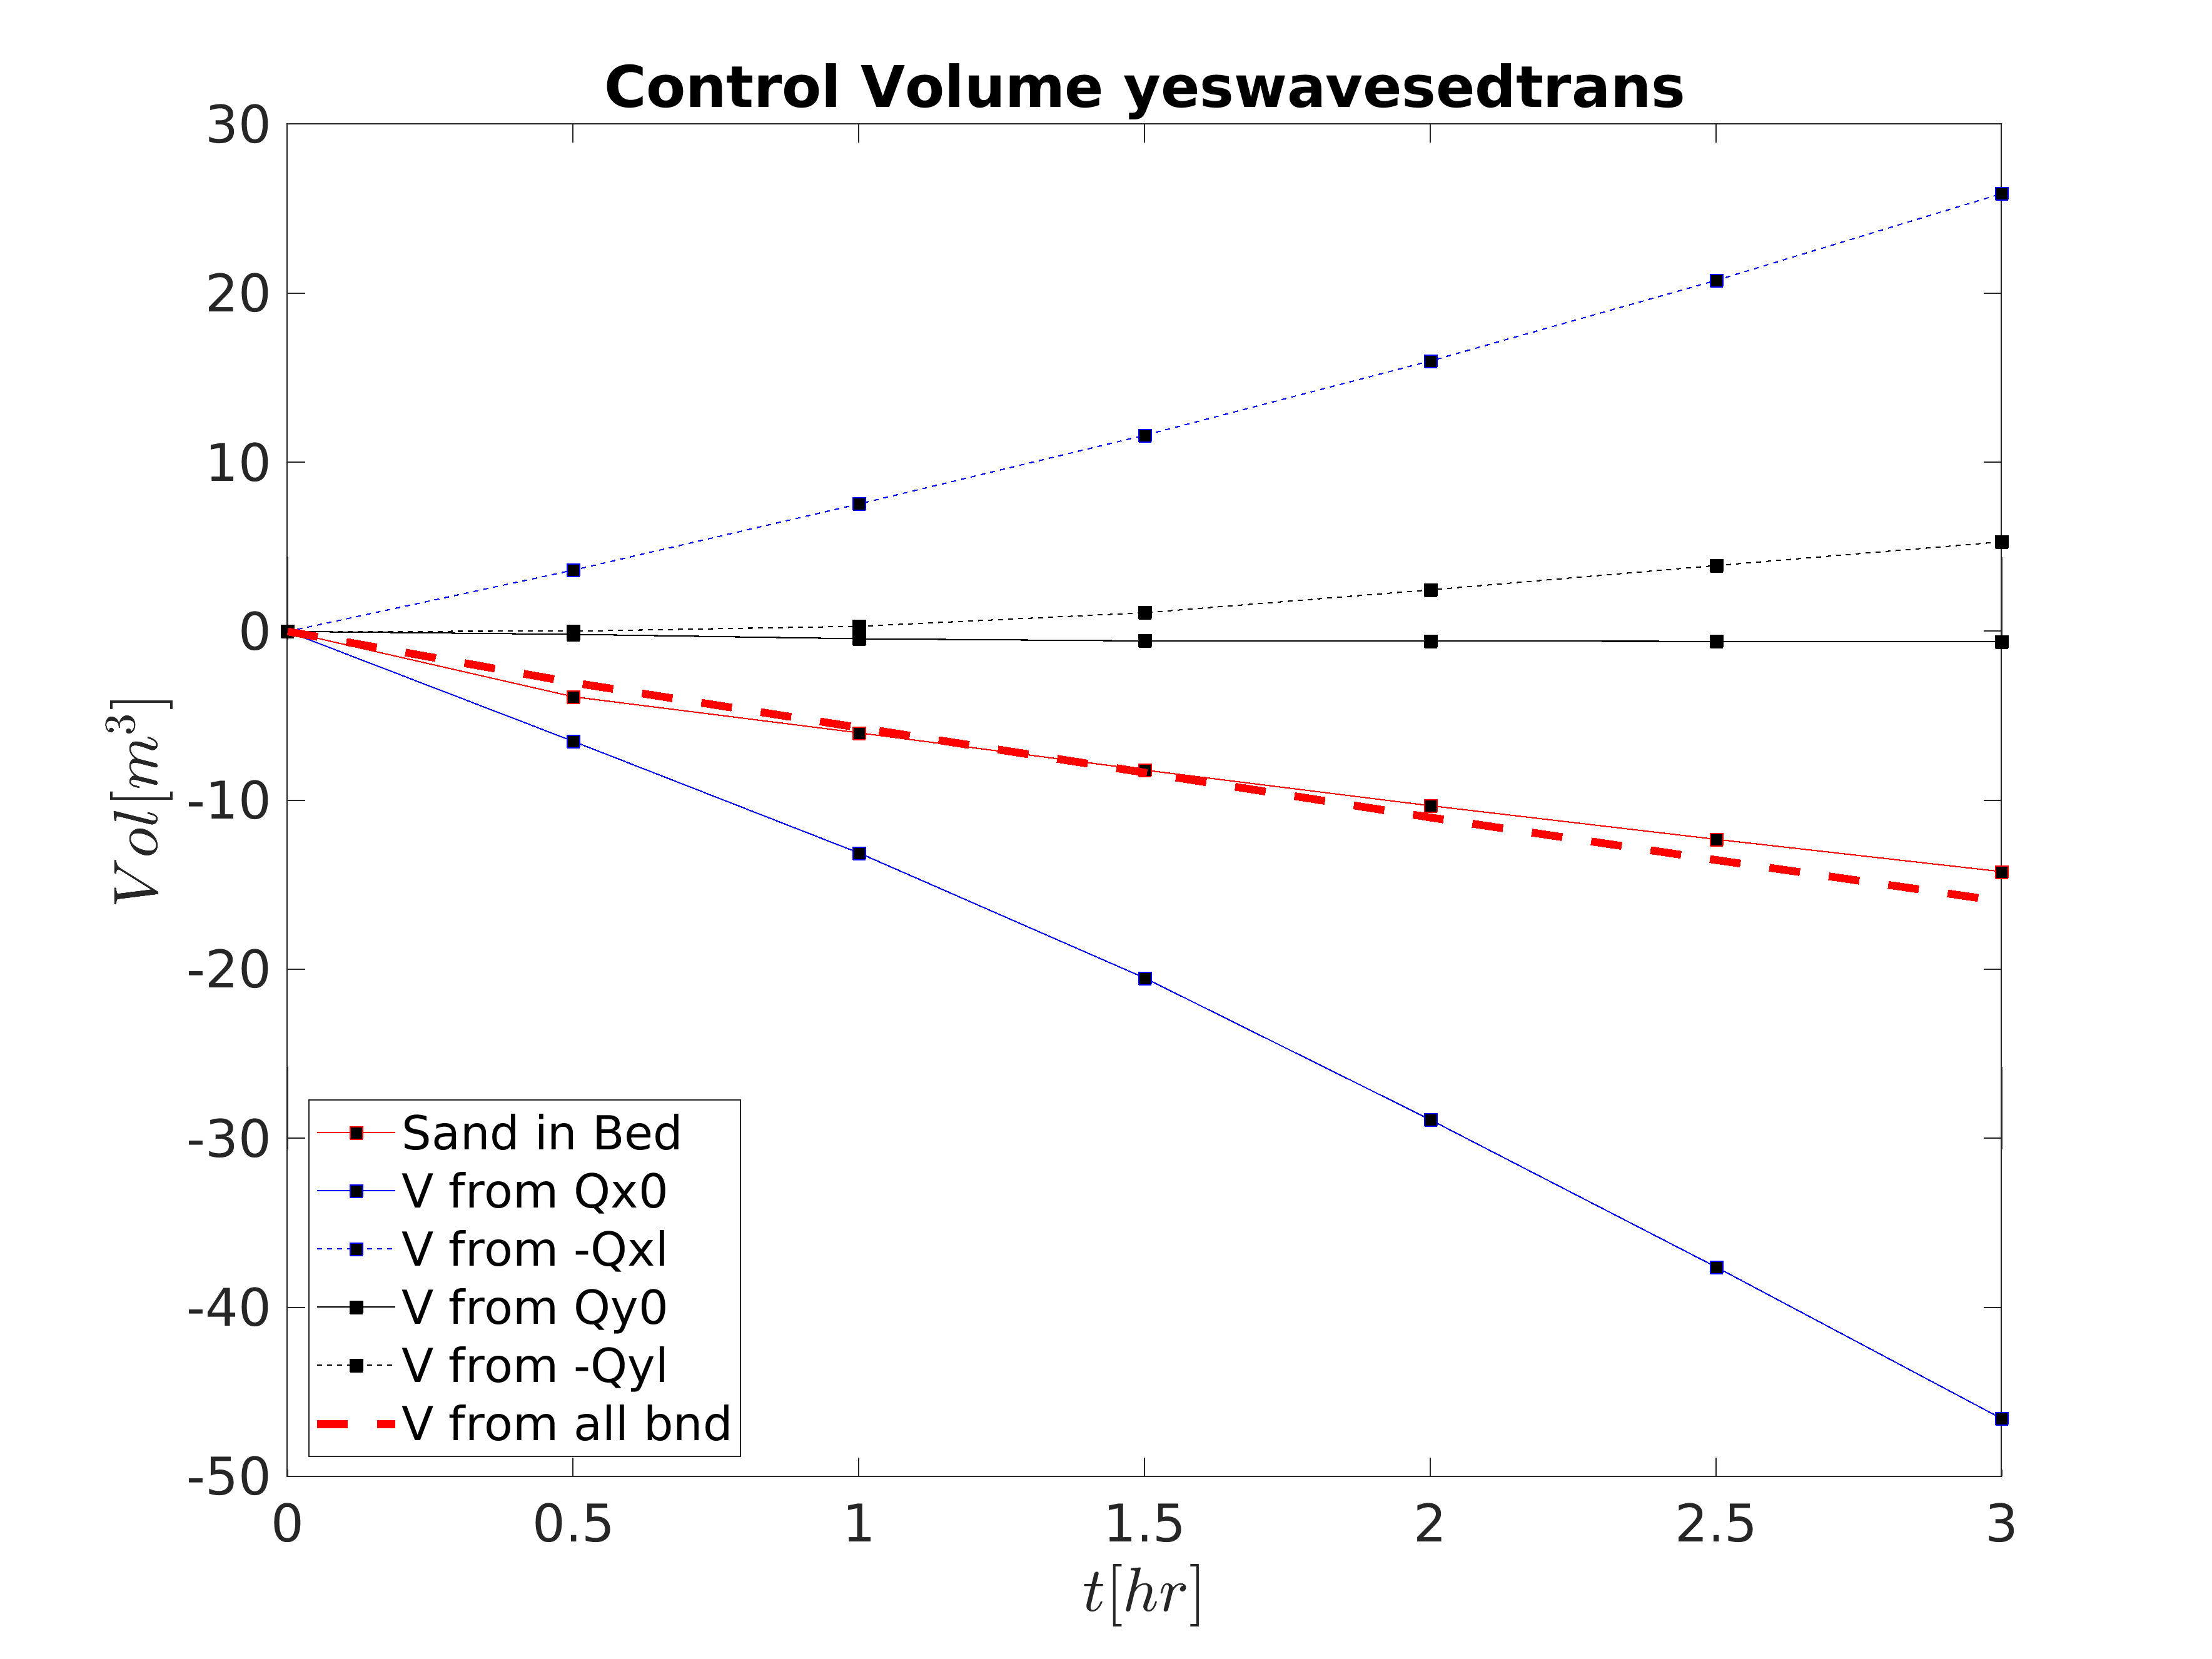
\includegraphics[width=.8\linewidth]{./control_vol_yeswavesedtrans.png}
  \end{center}
  \caption{Control Volume}
  \label{fig5}
\end{figure}

\clearpage
\section{CMS Formulation}
The {\verb NET } formulation of the CMS model has an time-dependent sed balance, provided here in one dimension, 
\begin{equation}
  \pdv{h c}{t} + \pdv{q_s}{x} = \alpha \omega_f \left\{c_* - c\right\}
\end{equation}
where $q_s = U h c$ is the advective transport. The sand conservation statement for a steady concentration field is given
\begin{equation}
  (1-p)  \pdv{z_b}{t} = -\pdv{q_s}{x}
\end{equation}
resulting in
\begin{equation}
  (1-p)  \pdv{z_b}{t} =  \alpha \omega_f \left\{c - c_*\right\}
\end{equation}

\section{CMS Formulation Proposed}
Returning to the sand conservation statement for a steady concentration field
\begin{equation}
  (1-p)  \pdv{z_b}{t} = -\pdv{q_s}{x} -\pdv{\tilde{q}}{x}
\end{equation}
where the transport is decomposed into a suspended portion and a
wave-driven component $\tilde{q}$.  It is proposed that we retain the
suspended balance and enforce the gradient of the wave driven transport
\begin{equation}
  (1-p)  \pdv{z_b}{t} =  \alpha \omega_f \left\{c - c_*\right\} -\pdv{\tilde{q_i}}{x_i}
\end{equation}
now provided in two dimensions.
This, essentially, presupposes that the wave-driven component reacts
instantaneously to the forcing and enforces mass-conservation of a
wave-driven transport vector.  Implementation will require returning
to the formulation in {\verb sediment.f90 } and parsing out the
advection and the additional terms, e.g. bedload, wave-related transport, swash transport, etc.

\end{document}




